\section{RQ3: Accuracy of Modeling Deployed Chatbots}

The goal of RQ3 is to evaluate \ac{TRACER} in a realistic environment,
using a black-box chatbot for which the ground truth is unknown.
Unlike the controlled environments of RQ1 and RQ2,
this evaluation uses publicly deployed, real-world chatbots.
The goal is to measure the precision of \ac{TRACER}'s inferred model,
defined as the percentage of discovered functionalities that are correct and valid.
We chose this metric over others, such as recall,
because we do not have access to the complete model.
Therefore, we cannot determine
if the inferred model is missing any functionality.

\subsection{Experiment Setup}

For this experiment, we selected five different real-world deployed chatbots.
Ada-UAM \autocite{AdaUAM},
Gallo de Morón de la Frontera \autocite{AyuntamientoMoronFrontera},
Madrid te Cuida \autocite{ChatbotMadridTe},
Gestri (Diputación de Valencia) \autocite{DiputacionAtiendeMas},
and Ayuntamiento de Arucas \autocite{AyuntamientoArucasASISTENTES}.

Ada-UAM is a university support chatbot.
Gallo de Morón de la Frontera and Ayuntamiento de Arucas
are citizen services chatbots for town halls.
Gestri offers a chatbot that assists with the payment of taxes.
Lastly, Madrid te Cuida offers sanitary assistance.

These chatbots were chosen because they represent
genuine production systems from various public sector domains.
All of them were easily accessible through an \ac{API}.

The first stage of the protocol was to execute \ac{TRACER}
against each of these five chatbots.
To maintain consistency with the previous research questions,
we ran \ac{TRACER} with 20 sessions, each with 12 turns,
and chose Gemini 2.0 Flash as the \ac{LLM}.

The second stage was the manual verification.
The verification was performed for each functionality
and it involved interacting with the chatbot
and validating that the chatbot exhibits that functionality.
We also checked for duplicate functionalities.
Based on this verification,
each of TRACER's discovered functionalities was classified
as either a \ac{TP} or a \ac{FP}.
With the results, we computed the precision
(see \autoref{eq:precision}),
a metric that measures the correctness and accuracy of
\ac{TRACER}'s output.

\begin{equation}
\label{eq:precision}
\text{Precision} = \frac{\mathrm{TP}}{\mathrm{TP} + \mathrm{FP}}
\end{equation}

\begin{itemize}
  \item \textbf{\acf{TP}:}
    The number of functionalities discovered by \ac{TRACER}
    that were confirmed to be real, valid, and distinct.
  \item \textbf{\acf{FP}:}
    The number of functionalities discovered by \ac{TRACER}
    that were either incorrect
    (not actually present in the chatbot)
    or were duplicates of another functionality.
\end{itemize}

\subsection{Results and Discussion}

\begin{figure}[!htb]
  \begin{center}
    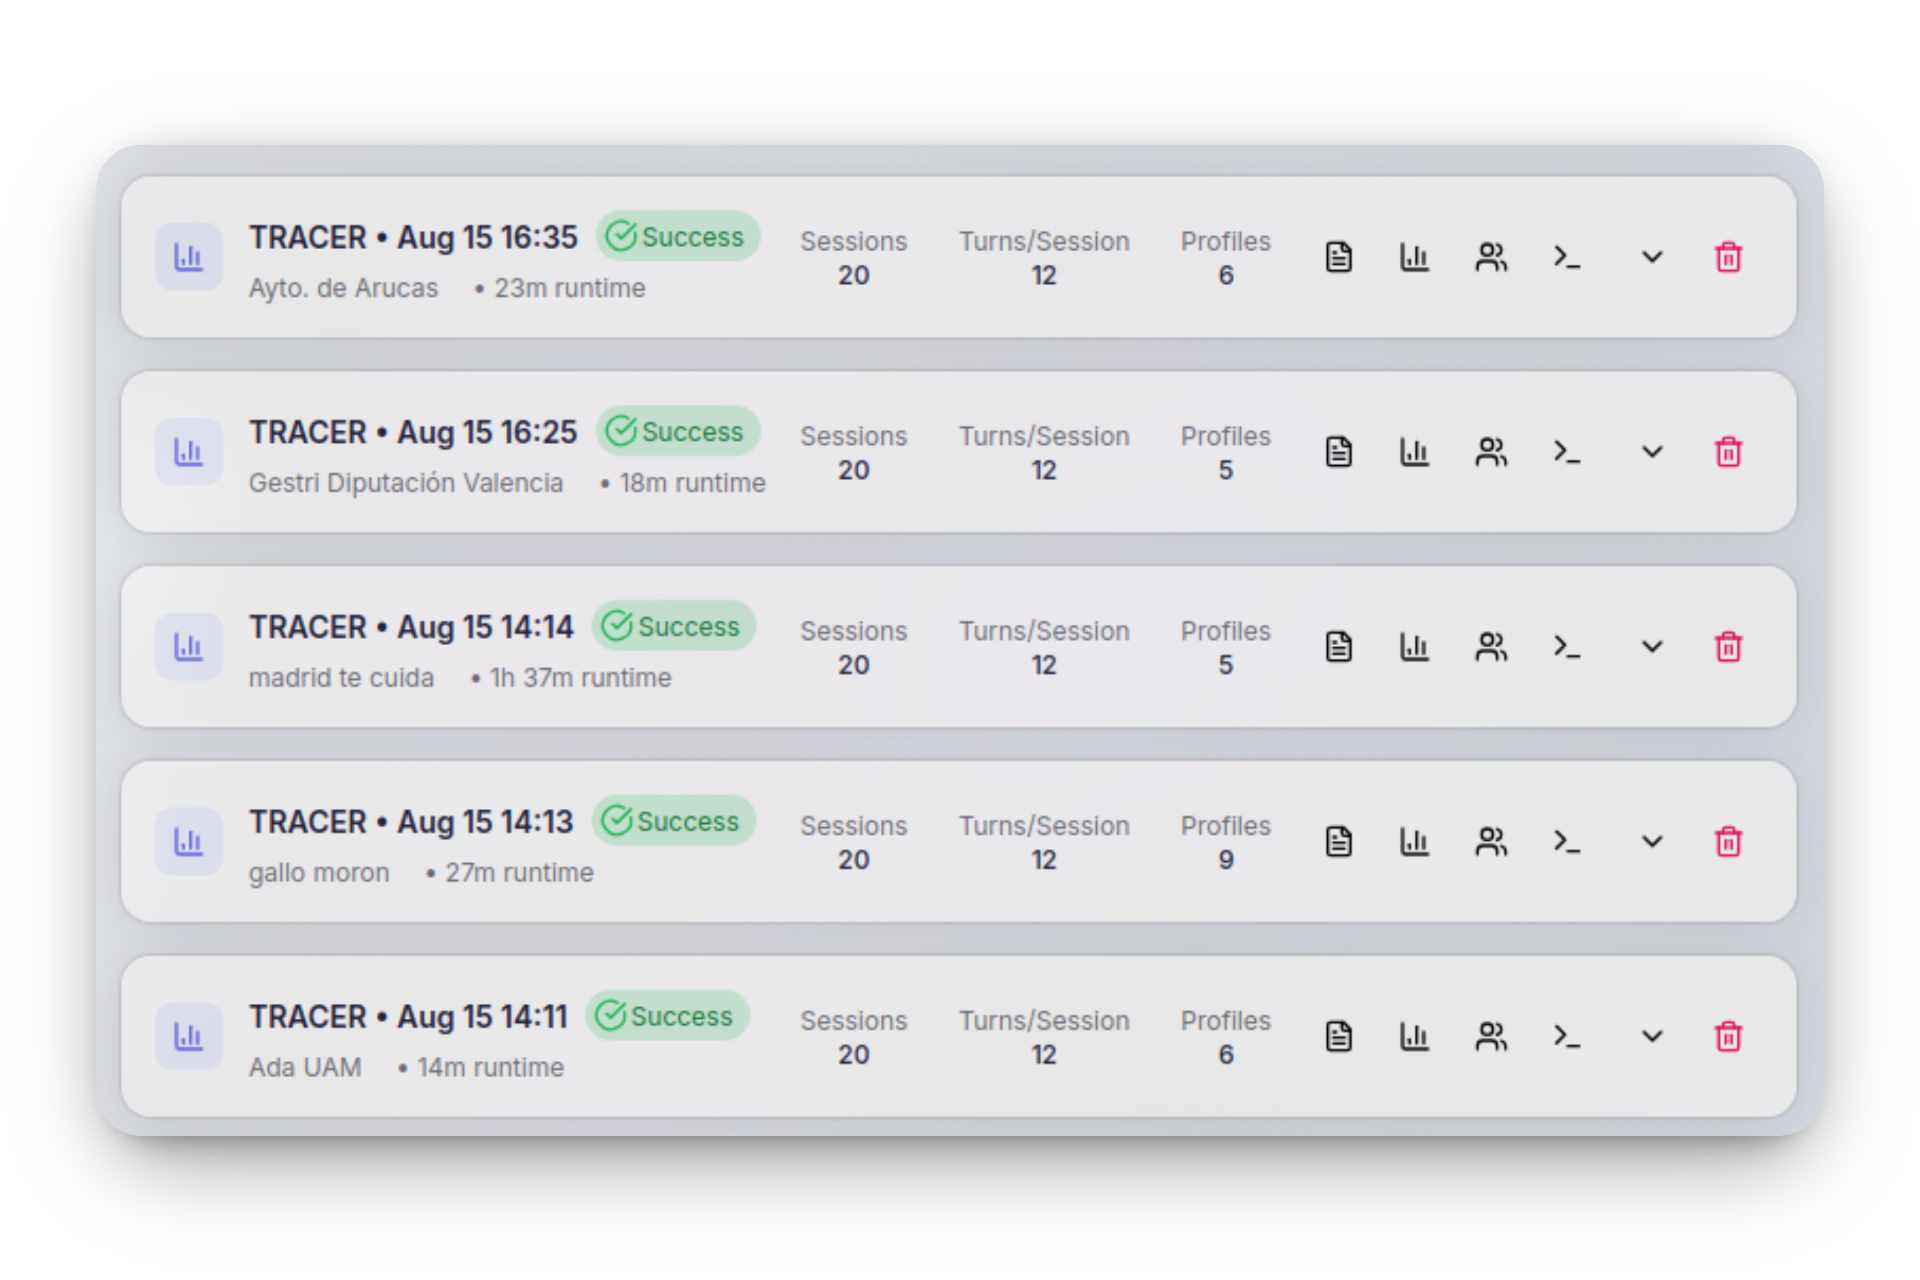
\includegraphics[width=\textwidth]{figures/tracer-results.png}
  \end{center}
  \caption{Screenshot of the web application showing
    the TRACER executions that contain the results of the experiment.}
  \label{fig:tracer-results}
\end{figure}

The inferred models by \ac{TRACER} can be found at
\url{http://miso.ii.uam.es:8081/tracer-dashboard}.
The screenshot in \autoref{fig:tracer-results}
shows the executions that contain the results of this experiment.
The projects are set to public
so that the results can be consulted
without needing to sign up on the web application.

\autoref{tab:rq3_precision_results}
summarizes the results of the manual verification for each of the five chatbots.
The table is divided into five columns; the first is the chatbot under testing.
\texttt{\# Func. (TRACER)} is the number of functionalities
found by \ac{TRACER}.
\texttt{\ac{TP}} is the number of those functionalities
that have been manually validated, i.e.,
the chatbot exhibits those functionalities
and are not duplicated.
Meanwhile, \texttt{\ac{FP}} represents those
that have been verified to be incorrect or duplicated.
Lastly, we have the \texttt{Precision} computed as shown in \autoref{eq:precision}.

\begin{table}[htpb]
\centering
\caption{Precision of TRACER's Inferred Models for Deployed Chatbots.}
\label{tab:rq3_precision_results}
\begin{tabular}{@{}lcccc@{}}
\toprule
\textbf{Chatbot} & \textbf{\thead{\# Func. \\ (TRACER)}} & \textbf{\thead{TP \\ (Verified)}} & \textbf{\thead{FP \\ (Incorrect/Duplicate)}} & \textbf{\thead{Precision (\%)}} \\ \midrule
Ada-UAM & 22 & 22 & 0 & 100.0 \\
Gallo de Morón & 29 & 27 & 2 & 93.1 \\
Madrid te Cuida & 91 & 88 & 3 & 96.7 \\
Gestri & 27 & 27 & 0 & 100.0 \\
Arucas & 41 & 37 & 4 & 90.2 \\ \midrule
\textbf{Total} & 210 & 201 & 9 & \textbf{96.0} \\ \bottomrule
\end{tabular}
\end{table}

An average precision of 96.0\% can be observed,
with a minimum of 90.2\% in the Arucas Town Hall chatbot.
A perfect score of a 100\% was achieved
on the simple chatbots Ada-UAM and Gestri.
And a 96.7\% was obtained in Madrid te Cuida,
the most complex chatbot tested with 91 discovered functionalities,
which 88 of them were verified to be valid and unique.

All but one of the \acp{FP} were duplicates.
This means that out of the 210 discovered functionalities,
only one was hallucinated,
i.e., 99.52\% of the functionalities
are real functionalities exhibited by the chatbot.
The hallucinated functionality was a claim that
Gallo de Morón offered a service to claim lottery prizes,
which it does not.
The remainder of the \acp{FP} were all duplicates
in which the LLM identified two very similar functionalities.
For example, in the 'Arucas' chatbot,
\ac{TRACER} created separate nodes for
'Present Electronic Office Options'
and 'Provide Electronic Office link'.
This indicates that while TRACER's discovery process is robust,
the automated consolidation logic can be further improved.

\subsection{Threats to Validity}
The evaluation of RQ3
is subject to threats concerning
both construct and external validity.

A threat to construct validity
is the inability to calculate recall.
This is a common challenge in black-box settings
where obtaining a ground-truth model is infeasible.
Therefore, while the precision of the inferred model
was effectively measured,
its completeness (recall) could not be
quantitatively assessed and remains an open question.

A second threat relates to external validity.
The evaluation, while using real-world systems,
is limited to five chatbots.
This small sample size
restricts the generalisability of the high precision scores.
Furthermore, the performance of TRACER
might differ when applied to more complex chatbots,
systems from other domains,
or agents operating primarily in languages other than those tested.

\subsection{Answer to RQ3}

The results of this experiment allow us to positively answer RQ3.
\ac{TRACER} demonstrated its ability
to accurately model the functionalities of
real-world, deployed chatbots, achieving an average precision of 96.0\%.
The qualitative analysis revealed that
the errors were not due to the hallucination of false functionalities
but rather to an over-granularity in distinguishing
between semantically similar features.
This confirms that \ac{TRACER} is a precise tool
to automatically model chatbots
in a black-box and real-world scenario.
